\documentclass[10pt]{article}
\usepackage[utf8]{inputenc}
\usepackage[english]{babel}
\usepackage[font=small,labelfont=bf]{caption}
\usepackage{geometry}
\usepackage[sort&compress, numbers]{natbib}
\usepackage{pxfonts}
\usepackage{graphicx}
\usepackage{setspace}
\usepackage{hyperref}
\usepackage{lineno}

\newcommand{\demo}{S1}

\doublespacing
\linenumbers

\title{Geometric models reveal the hidden structure of conceptual knowledge}

\author{Paxton C. Fitzpatrick\textsuperscript{1} and Jeremy R.
Manning\textsuperscript{*, 1}\\\textsuperscript{1}Dartmouth
College\\\textsuperscript{*}Corresponding author:
jeremy.r.manning@dartmouth.edu}

\date{}

\begin{document}
\maketitle

\begin{abstract} We develop a mathematical framework, based on natural language
processing models, for tracking and characterizing the acquisition of
conceptual knowledge. Our approach embeds each concept in a high dimensional
representation space, where nearby coordinates reflect similar or related
concepts. We tested our approach using behavioral data collected from a group
of college students. In the experiment, we asked the participants to answer
sets of quiz questions interleaved between watching two course videos from the
Khan Academy platform. We applied our framework to the videos' transcripts, and
to text of the quiz questions, to quantify the content of each moment of video
and each quiz question. We used these embeddings, along with participants' quiz
responses, to track how the learners' knowledge changed after watching each
video. Our findings show how a limited set of quiz questions may be used to
construct rich and meaningful representations of what each learner knows, and
how their knowledge changes over time as they learn.

\textbf{Keywords: education, learning, knowledge, concepts, natural language processing}

\end{abstract}


\section*{Introduction}

How do we acquire conceptual knowledge? Memorizing course lectures or textbook
chapters by rote can lead to the superficial \textit{appearance} of
understanding the underlying content, but achieving true conceptual
understanding seems to require something deeper and richer. Does conceptual
understanding entail connecting newly acquired information to the scaffolding
of one's existing knowledge or experience? Or weaving a lecture's atomic
elements (e.g., its component words) into a structured network that describes
how those individual elements are related? Conceptual understanding could also
involve building a mental model that transcends the meanings of those
individual atomic elements by reflecting the deeper meaning underlying the
gestalt whole.

The difference between ``understanding'' and ``memorizing,'' as framed by the
researchers in education, cognitive psychology, and cognitive
neuroscience~\citep{Kato40, Gall10, ScotEtal13, HallGree08, Macl05} has
profound analogs in the fields of natural language processing and natural
language understanding. For example, considering the raw contents of a document
(e.g., its constituent symbols, letters, and words) might provide some
information about what the document is about, just as memorizing a passage
might be used to answer simple questions about the passage~\citep[e.g., whether
it might contain words related to furniture versus physics;][]{LandDuma97,
BleiEtal03, BleiLaff06}. However, modern natural language processing
models~\citep[e.g.,][]{MikoEtal13a, CerEtal18, BrowEtal20} also attempt to
capture the deeper meaning \textit{underlying} those atomic elements. These
models consider not only the co-occurrences of those elements within and across
documents, but also patterns in how those elements appear across different
scales (e.g., sentences, paragraphs, chapters, etc.), the temporal and
grammatical properties of the elements, and other high-level characteristics of
how they are used~\citep{Mann20, Mann21a}. According to these models, the deep
conceptual meaning of a document may be captured by a feature vector in a
high-dimensional representation space, where nearby vectors reflect
conceptually related documents. A model that succeeds at capturing an analog of
``understanding'' is able to assign nearby feature vectors to two conceptually
related documents, \textit{even when the words contained in those documents
have very little overlap}.

What form might the representation of the sum total of a person's knowledge
take? First, we might require a means of systematically describing or
representing the nearly infinite set of possible things a person could know.
Second, we might want to account for potential associations between different
concepts. For example, the concepts of ``fish'' and ``water'' might be
associated in the sense that fish live in water. Third, knowledge may have a
critical dependency structure, such that knowing about a particular concept
might require first knowing about a set of other concepts. For example,
understanding the concept of a fish swimming in water first requires
understanding what fish and water \textit{are}. Fourth, as we learn, our
``current state of knowledge'' should change accordingly. Learning new concepts
should both update our characterizations of ``what is known'' and should also
unlock any now-satisfied dependencies of that newly learned concept so that
they are ``tagged'' as available for future learning.

Here we develop a framework for modelling how knowledge is acquired during
learning. The central idea is to use text embedding models to define the
coordinate systems of two maps: (a) a \textit{knowledge map} that describes the
extent to which each concept is currently known and (b) a \textit{learning map}
that describes the extent to which each concept could be learned. Each location
on these maps represents a single concept, and the geometries are defined such
that related concepts are located nearby in space. We use this framework to
analyzing and interpreting behavioral data collected from an experiment that
has participants watch and answer conceptual questions about a series of
recorded course lectures.

Our primary research goal is to advance our understanding of what it means to
acquire deep real-world conceptual knowledge. Traditional laboratory approaches
to studying learning and memory (e.g., list learning studies) often draw little
distinction between memorization and understanding. Instead, these studies
typically focus on whether information is effectively encoded or retrieved,
rather than whether the information is \textit{understood}. Approaches to
studying conceptual learning, such as category learning experiments, can start
to investigate the distinction between memorization and understanding, often by
training participants to distinguish arbitrary or random features in otherwise
meaningless categorized stimuli. However the objective of real-world training,
or learning from life experiences more generally, is often to develop new
knowledge that may be applied in \textit{useful} ways in the future. In this
sense, the gap between modern learning theories and modern pedagogical
approaches and classroom learning strategies is enormous: most of our theories
about \textit{how} people learn are inspired by experimental paradigms and
models that have only peripheral relevance to the kinds of learning that
students and teachers actually seek. To help bridge this gap, our study uses
course materials from real online courses to inform, fit, and test models of
real-world conceptual learning.

\section*{Results}

\begin{figure}[tp]
\centering
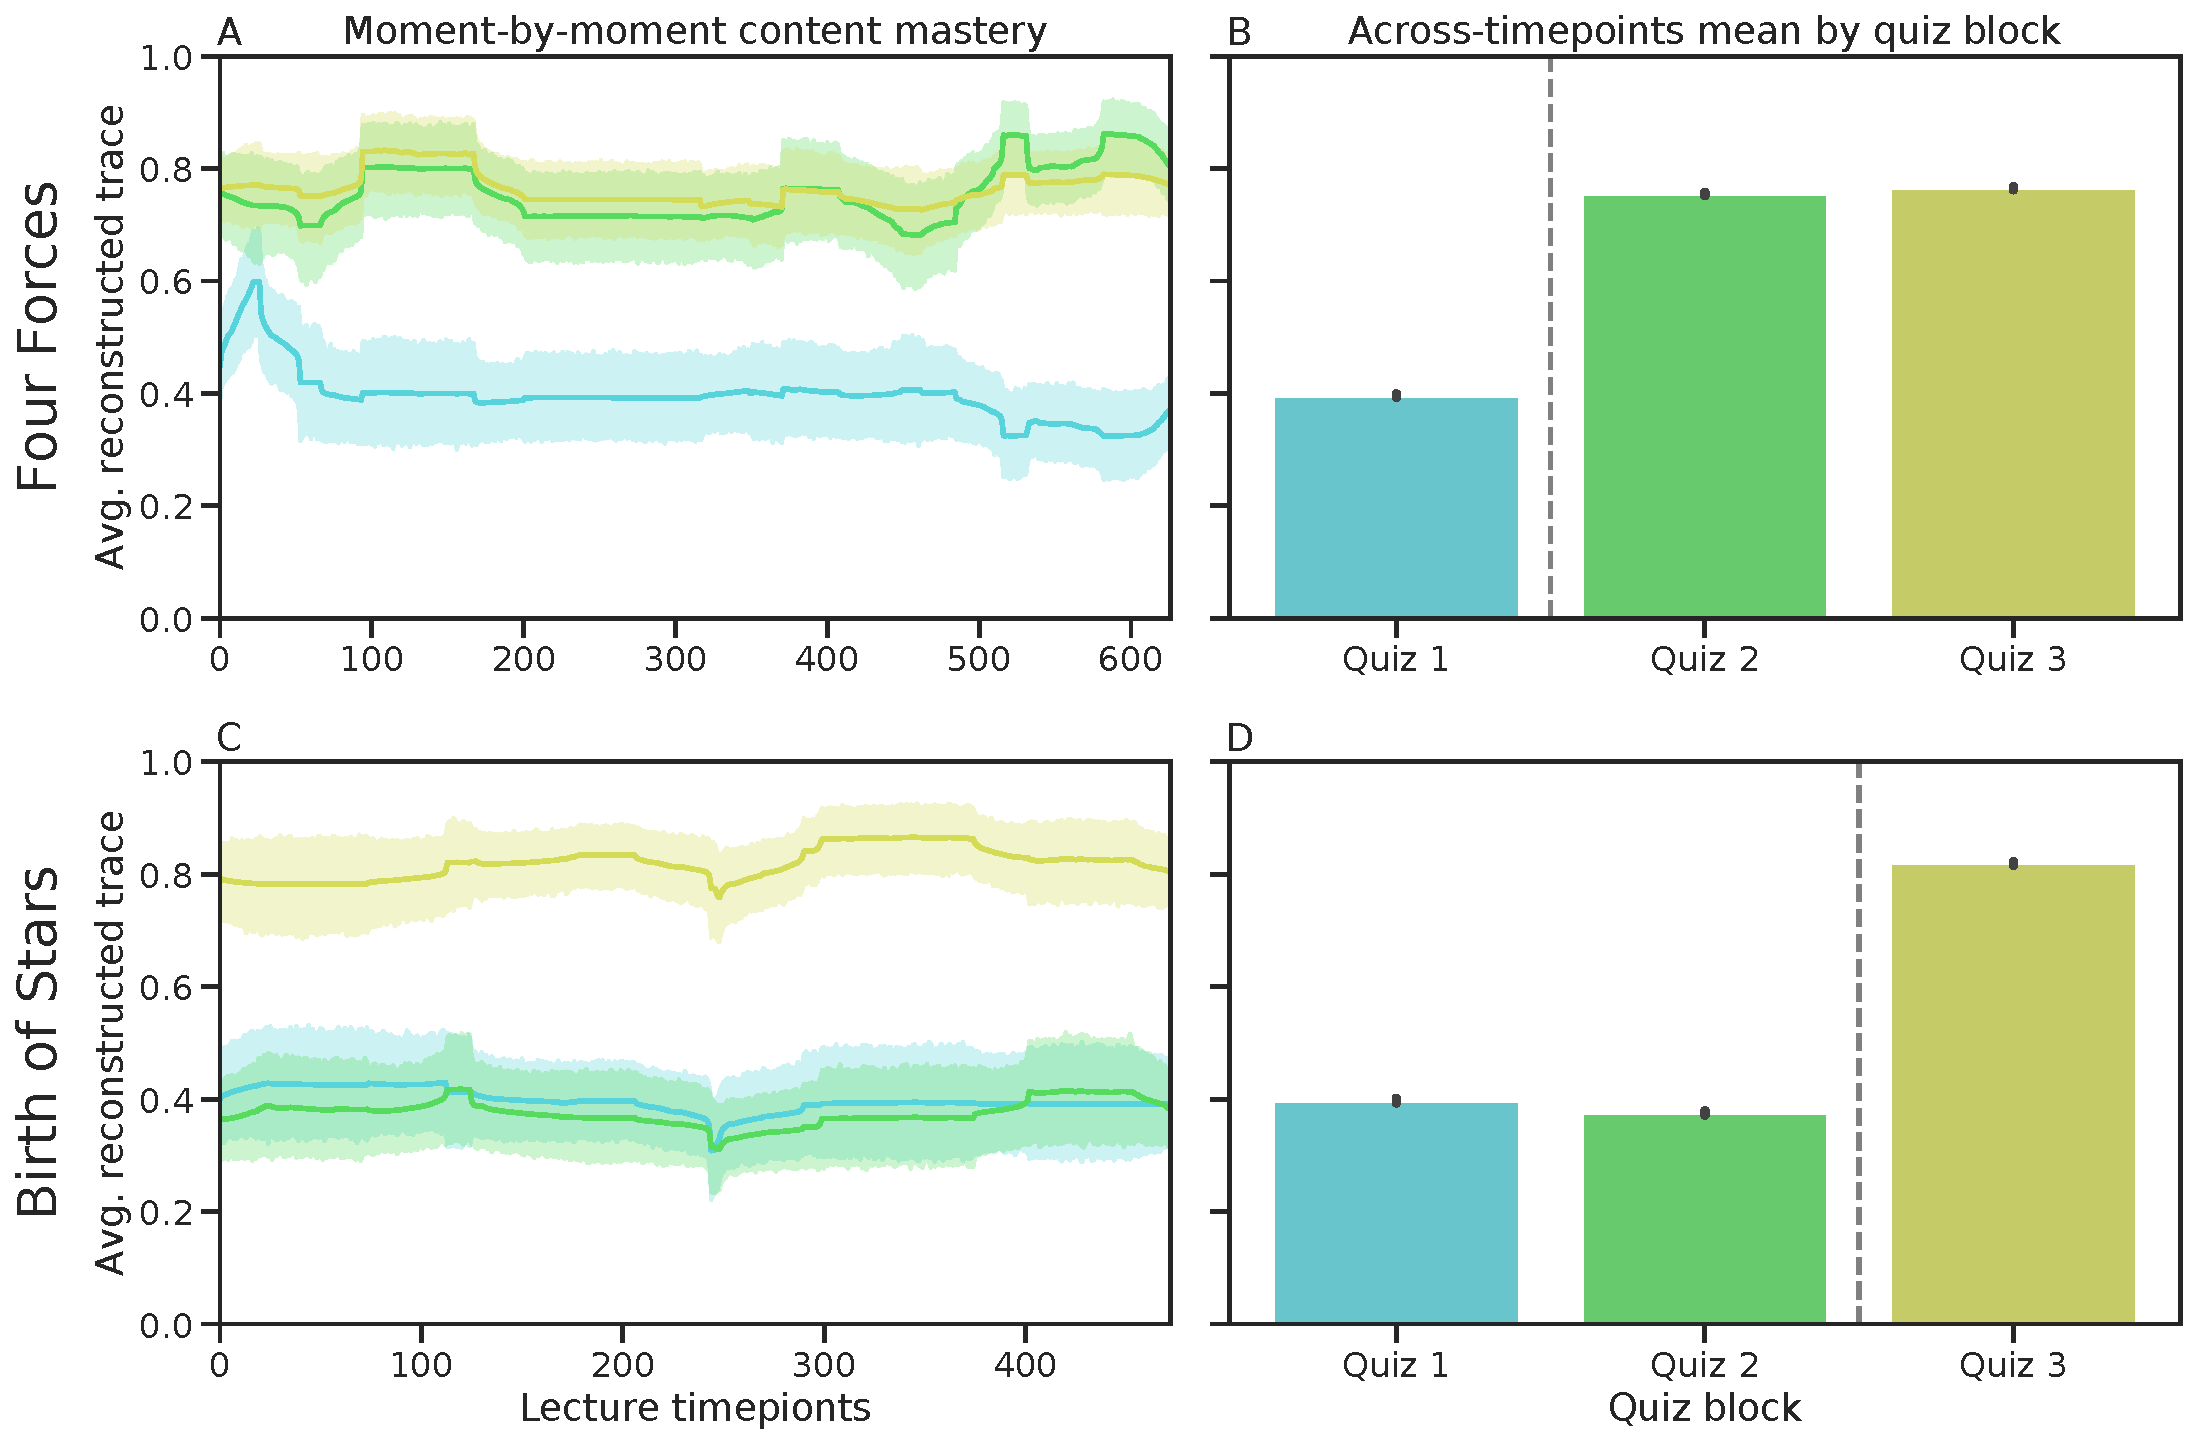
\includegraphics[width=0.8\textwidth]{figs/content-mastery}
\caption{\textbf{Caption.} Placeholder text.}
\label{fig:demo}
\end{figure}

\section*{Discussion}

\section*{Materials and methods}

\subsection*{Participants}

\subsection*{Experiment}

\subsection*{Analysis}

\subsubsection*{Constructing text embeddings of multiple videos and questions}

\subsubsection*{Estimating held-out conceptual knowledge}

\subsubsection*{Creating knowledge and learning map visualizations}



\bibliographystyle{apa}
\bibliography{CDL-bibliography/cdl}
\end{document}
